\clearpage
\chapter{Experiments}
Chapter 3 described how the experiments will be executed and Chapter 4 described the subjects of the tests, algorithms and software. This chapter contains the results of these experiments. Each of the sections will contain graphs and tables showcasing the results, alongside a brief description of the numbers produced. 
\clearpage
\section{Quicksort}

\clearpage
\section{Mandelbrot}
Mandelbrot algorithm experiments were conducted using parameters presented in Tab. \ref{tab: MandelbrotParameters}. They describe amount of pixels generated and bitmap dimensions.
Sequential version of the algorithm had a MET  $\approx 5.6s$ . Parallel counterpart clocked at MET  $\approx 2.1s$, for a $\approx 62\%$ reduction. Parallel version with two \emph{Parallel.For} loops had a MET $\approx 2.7s$ which is $\approx 21\%$ slower than the less parallelized version using only one parallel loop. The best performing version using value type complex number had MET $\approx 1.9s$, for a $\approx 66\%$  reduction compared to sequential version and $\approx 11\%$  reduction to the parallel version. Additionaly, the value type version had 0 GC clean ups and virtually no (compared to others) memory consumption (Fig. \ref{fig: MandelbrotPerformance}, Tab. \ref{tab: MandelbrotBenchmarking}).

\begin{table}[!ht]
    \centering
    \caption{Mandelbrot benchmarking experiment parameters}
		\label{tab: MandelbrotParameters}
    \begin{tabular}{p{3cm}p{3cm}}
			\toprule
			\bfseries Name 	&
			\bfseries Value \\
			\midrule
			Width & 2.5 \\
			Height & 2.5 \\
			Column amount & 4000 \\ 
			Row amount  & 4000 \\	
			\bottomrule
    \end{tabular}
\end{table}

\begin{figure}[htb]
\centering
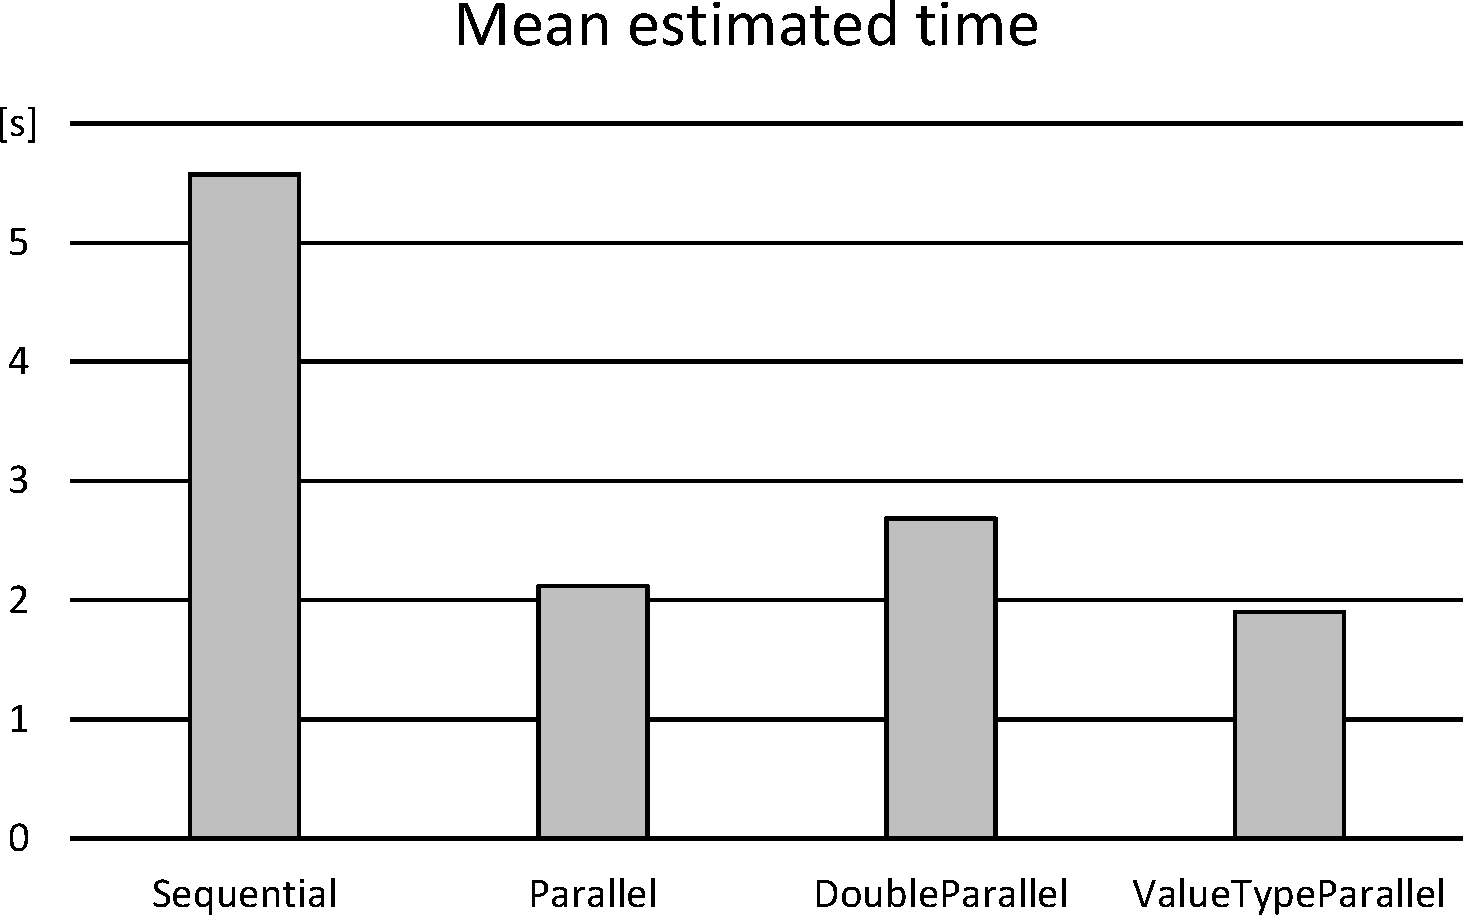
\includegraphics[width=.8\linewidth]{figures04/Fig41.pdf}
%%\begin{tikzpicture}
%%\begin{axis}[ symbolic x coords={
			%%Sequential, 
			%%Parallel, 
			%%DoubleParallel, 
			%%ValueTypeParallel, 
			%%DUMMY},
    %%xtick=data, 
		%%ylabel=Seconds,
    %%ybar interval=.7,
    %%enlargelimits=0.05]
    %%\addplot  coordinates {
      %%(Sequential, 5.576)
      %%(Parallel, 2.120)
      %%(DoubleParallel, 2.684)
      %%(ValueTypeParallel,1.903)
      %%(DUMMY, 0)
    %%};
     %%\legend{Mean estimated time}
%%\end{axis}
%%\end{tikzpicture}
\caption{Mandelbrot algorithm performance}
\label{fig: MandelbrotPerformance}
\end{figure}

\begin{table}[ht]%\small
    \centering
    \caption{Mandelbrot benchmarking results}
		\label{tab: MandelbrotBenchmarking}
    \begin{tabularx}{\linewidth}{Xrrrrrrr} \toprule
			\bfseries Version 	&
			\bfseries Mean    	&
			\bfseries Error	    &
			\bfseries StdDev	  &
			\bfseries Gen 0	    &
			\bfseries Gen 1	    &
			\bfseries Gen 2	    &
			\bfseries Allocated \\ \midrule
			Sequential & 5.576 s & 0.0564 s & 0.0528 s & 2483000 & 1000 & 1000 & 19851 MB \\ 
			Parallel & 2.120 s & 0.0458 s & 0.1350 s & 2485000 & 6000 & 1000 & 19843 MB \\ 
			DoubleParallel & 2.684 s & 0.0553 s & 0.1632 s & 2487000 & 39000 & 2000 & 19852 MB \\ 
			ValueTypeParallel & 1.903 s & 0.0137 s & 0.0128 s & 0 & 0 & 0 & 46 MB \\ 
			\bottomrule
	\end{tabularx}
\end{table}

\clearpage
\section{K-means clustering}
K-means clustering algorithm experiments were conducted using \emph{White wine quality} dataset \cite{WhiteWine}. Sequential version of the algorithm had MET $\approx 2.45s$ while the parallel one had MET $\approx 0.5s$, for a $\approx 80\%$ reduction at the cost of $\approx 18\%$ increase of memory consumption. Using partitioner further dropped down the MET to $\approx 0.43s$ which is a $\approx 82\%$ reduction from the sequential version and $\approx 15\%$ from the parallel one with equal memory consumption increase (Fig. \ref{fig: KMeansPerformance}, Fig. \ref{fig: KMeansMemory}, Tab. \ref{tab: KMeansBenchmarking}).

\begin{figure}[!ht]
\centering
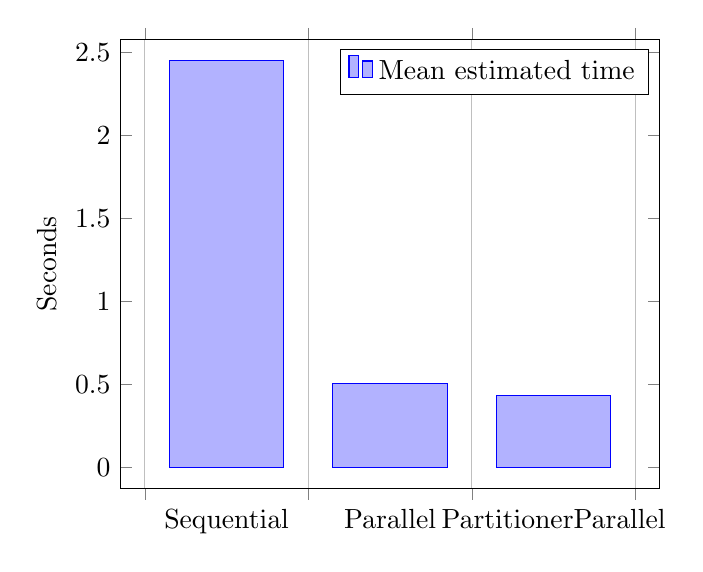
\begin{tikzpicture}
\begin{axis}[ symbolic x coords={
			Sequential, 
			Parallel, 
			PartitionerParallel, 
			DUMMY},
    xtick=data, 
		ylabel=Seconds,
    ybar interval=.7,
    enlargelimits=0.05]
    \addplot  coordinates {
      (Sequential, 2.4537)
      (Parallel, 0.5096)
      (PartitionerParallel, 0.4345)
      (DUMMY, 0)
    };
     \legend{Mean estimated time}
\end{axis}
\end{tikzpicture}
\caption{K-means clustering  performance}
\label{fig: KMeansPerformance}
\end{figure}

\begin{figure}[!ht]
\centering
\begin{tikzpicture}
\begin{axis}[ symbolic x coords={
			Sequential, 
			Parallel, 
			PartitionerParallel, 
			DUMMY},
    xtick=data, 
		ylabel=Megabytes,
    ybar interval=.7,
    enlargelimits=0.05]
    \addplot[fill=gold]  coordinates {
      (Sequential, 151)
      (Parallel, 183)
      (PartitionerParallel, 184)
      (DUMMY, 0)
    };
     \legend{Memory consumption}
\end{axis}
\end{tikzpicture}
\caption{K-means clustering memory consumption}
\label{fig: KMeansMemory}
\end{figure}

\begin{table}[ht]%\small
    \centering
    \caption{K-means clustering benchmarking results}
		\label{tab: KMeansBenchmarking}
    \begin{tabularx}{\linewidth}{Xrrrrrrr} \toprule
			\bfseries Version 	&
			\bfseries Mean    	&
			\bfseries Error	    &
			\bfseries StdDev	  &
			\bfseries Gen 0	    &
			\bfseries Gen 1	    &
			\bfseries Gen 2	    &
			\bfseries Allocated \\ 
			\midrule 
Sequential & 2,453.7 ms	& 25.01ms	& 20.89ms	& 18000 & 	2000 & 	0 & 151 MB \\
Parallel & 509.6 ms	& 8.28 ms	& 8.50 ms	& 23000 & 	9000 & 	0 & 183 MB \\ 
PartitionerParallel & 434.5 ms	& 2.69 ms	& 2.52 ms	& 23000 & 	8000 & 	0 & 184 MB \\
			\bottomrule
		\end{tabularx}
\end{table}
		
\clearpage
\section{Nuget package ranking}
Nuget package ranking software was tested using 3 datasets varying in size, other parameters were constast across tests (Tab. \ref{tab: NuGetParameters}). \\
When testing with the small dataset, sequential version had MET $\approx 1.7s$, while parallel one had MET $\approx 0.35s$ for a $\approx 79\%$ reduction. In this case, usage of partitioner worsened the performance with MET  $\approx 0.38s$, which is $\approx 6\%$ slower. \\ 
During tests with the medium dataset, sequential version had MET $\approx 17.5s$. Parallel version clocket at $\approx 4.6s$, for a $\approx 76\%$ reduction. This time partitioner version improved the performance at MET $\approx 3s$, which is $\approx 35\%$ faster than the bare parallel counterpart. \\ 
Finally sequential version on the large dataset had MET $\approx 56.9s$ while the parallel one had MET $\approx 14.4s$ which is $\approx 75\%$ less.
The partitioner continued the reducing trend at MET $\approx 9.4s$, improving the parallel version by $\approx 42 \%$. \\
Across all dataset the parallel version observed increase of memory consumption of $\approx 14\%$.

\begin{table}[!ht]
    \centering
    \caption{Nuget package ranking experiments parameters}
		\label{tab: NuGetParameters}
    \begin{tabular}{p{5cm}p{3cm}}
			\toprule
			\bfseries Name 	&
			\bfseries Value &
			\midrule
			\emph{Map} degree of parallelism & 10 \\
			\emph{Reduce} degree of parallelism & 10 \\
			Iterations & 10 \\ 
			Small dataset  & 1000 packages  \\	
			Medium dataset  & 5000 packages  \\	
			Large dataset  & 10000 packages  \\	
			\bottomrule
    \end{tabular}
\end{table}

\begin{figure}[!ht]
\centering
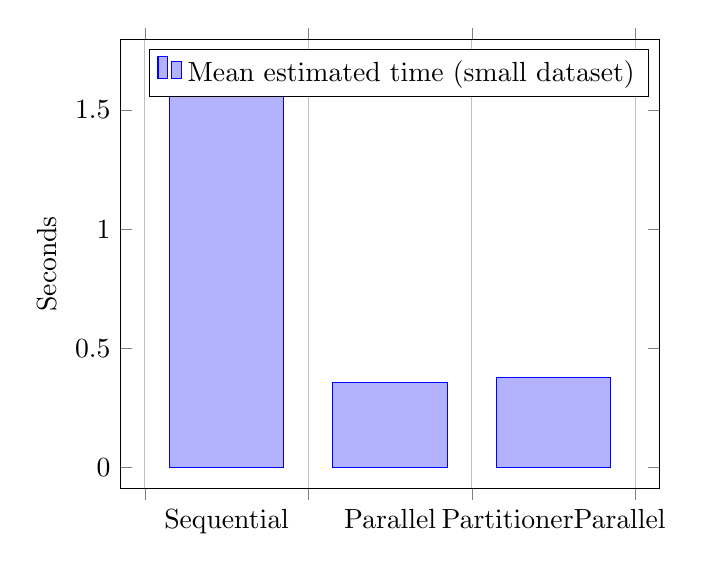
\begin{tikzpicture}
\begin{axis}[ symbolic x coords={
			Sequential, 
			Parallel, 
			PartitionerParallel, 
			DUMMY},
    xtick=data, 
		ylabel=Seconds,
    ybar interval=.7,
    enlargelimits=0.05]
    \addplot  coordinates {
      (Sequential, 1.709)
      (Parallel, 0.357)
      (PartitionerParallel, 0.380)
      (DUMMY, 0)
    };
     \legend{Mean estimated time (small dataset)}
\end{axis}
\end{tikzpicture}
\caption{NuGet package ranking performance - small dataset}
\label{fig: KMeansPerformanceSmall}
\end{figure}

\begin{figure}[!ht]
\centering
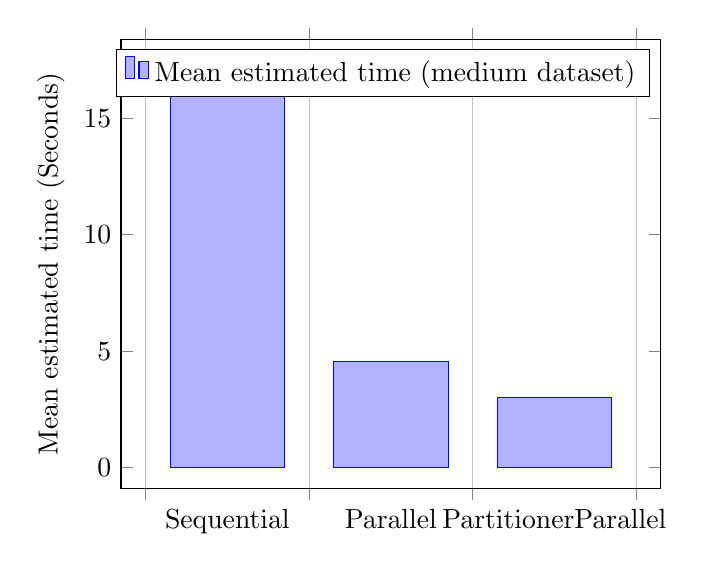
\begin{tikzpicture}
\begin{axis}[ symbolic x coords={
			Sequential, 
			Parallel, 
			PartitionerParallel, 
			DUMMY},
    xtick=data, 
		ylabel= Mean estimated time (Seconds),
    ybar interval=.7,
    enlargelimits=0.05]

		 \addplot  coordinates {
      (Sequential, 17.491)
      (Parallel, 4.564)
      (PartitionerParallel, 3.007)
      (DUMMY, 0)
    };
     \legend{Mean estimated time (medium dataset)}
\end{axis}
\end{tikzpicture}
\caption{NuGet package ranking performance - medium dataset}
\label{fig: KMeansPerformanceMedium}
\end{figure}

\begin{figure}[!ht]
\centering
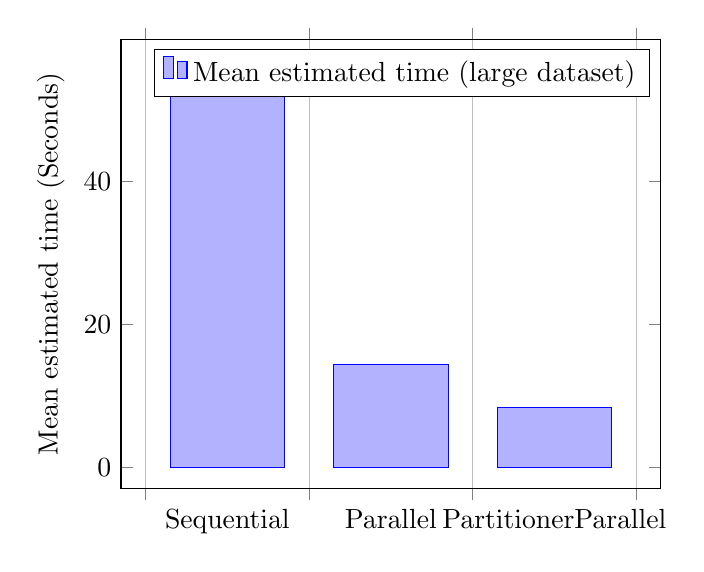
\begin{tikzpicture}
\begin{axis}[ symbolic x coords={
			Sequential, 
			Parallel, 
			PartitionerParallel, 
			DUMMY},
    xtick=data, 
		ylabel= Mean estimated time (Seconds),
    ybar interval=.7,
    enlargelimits=0.05]

		 \addplot  coordinates {
      (Sequential, 56.909)
      (Parallel, 14.377)
      (PartitionerParallel, 8.428)
      (DUMMY, 0)
    };
     \legend{Mean estimated time (large dataset)}
\end{axis}
\end{tikzpicture}
\caption{NuGet package ranking performance - large dataset}
\label{fig: KMeansPerformanceMedium}
\end{figure}

\begin{figure}[!ht]
\centering
\begin{tikzpicture}
\begin{axis}[ symbolic x coords={
			Sequential, 
			Parallel, 
			PartitionerParallel, 
			DUMMY},
    xtick=data, 
		ylabel=Megabytes,
    ybar interval=.7,
    enlargelimits=0.05]
    \addplot[fill=gold]  coordinates {
      (Sequential, 19)
      (Parallel, 22)
      (PartitionerParallel, 23)
      (DUMMY, 0)
    };
		\addplot coordinates {
      (Sequential, 57)
      (Parallel, 65)
      (PartitionerParallel, 65)
      (DUMMY, 0)
    };
		\addplot coordinates {
      (Sequential, 99)
      (Parallel, 114)
      (PartitionerParallel, 114)
      (DUMMY, 0)
    };
     \legend{Small dataset, Medium dataset}
\end{axis}
\end{tikzpicture}
\caption{NuGet package ranking memory consumption}
\label{fig: NugetMemory}
\end{figure}

\begin{table}[!ht]
    \centering
    \caption{K-means clustering benchmarking results}
		\label{tab: KMeansBenchmarking}
    \begin{tabularx}{\linewidth}{Xrrrrrrr} \toprule
			\toprule
			\bfseries Version 	&
			\bfseries Mean    	&
			\bfseries Error	    &
			\bfseries StdDev	  &
			\bfseries Gen 0	    &
			\bfseries Gen 1	    &
			\bfseries Gen 2	    &
			\bfseries Allocated &
			\midrule 
			\multicolumn{8}{c}{Small dataset} \\ 
			\midrule
			Sequential & 1,709.1 ms	& 4.71 ms	& 4.17 ms	& 2000 & 0 &    0 &	19 MB \\
			Parallel & 357.3 ms	& 7.55 ms	& 12.61 ms	& 2000 & 1000 &	0 &	22 MB \\
			PartitionerParallel & 380.5 ms	& 6.51 ms	& 10.33 ms	& 2000 & 1000 &	0 
&	23 MB \\
			\midrule
			\multicolumn{8}{c}{Medium dataset} \\ 
			\midrule
			Sequential & 17.491 s     &  0.2455 s &	0.2296 s& 7000 & 3000 &	0 &	57 
MB \\
			Parallel & 4.564 s	     & 0.0684 s	 &0.0606 s	& 8000 & 4000 &	0 &	65 
MB \\
			PartitionerParallel & 3.007 s	     & 0.0577 s	 &0.0730 s	& 8000 & 3000 
&	0 &	65 MB \\
			\midrule
      \multicolumn{8}{c}{Large dataset} \\ 
			\midrule
			Sequential    &      56.909 s &	0.6018 s &	0.5630 s &	12000 & 	5000 
&	0	& 99 MB  \\
			Paralllel     &      14.377 s &	0.0644 s &	0.0571 s &	14000 &	5000	 &
 0	& 114 MB \\
			PartitionerParallel &  8.428 s  &	0.0359 s &	0.0300 s &	14000 &	5000	 &
 0	& 114 MB \\
			\bottomrule
    \end{tabularx}
\end{table}

All experiments were properly displayed and described. Next chapter will discuss the implications of these results and formulate a set of guidelines based on them. 


